\chapter{Work Plan}
\label{chap:WorkPlan}

The execution of this dissertation followed a structured 12-month plan, commencing in November 2024 and culminating in the submission in October 2025. This chapter outlines the strategic phasing of the project, designed to ensure a logical progression from foundational research to final implementation and evaluation.

The timeline was organized into five distinct but overlapping phases, each with specific objectives and deliverables. This approach facilitated agile adaptation while maintaining a clear focus on the project's long-term goals. The complete project schedule, including granular tasks and their dependencies, is visualized in the Gantt chart presented in Figure~\ref{fig:gantt_chart_detailed}.

\begin{figure}[htbp]
    \centering
    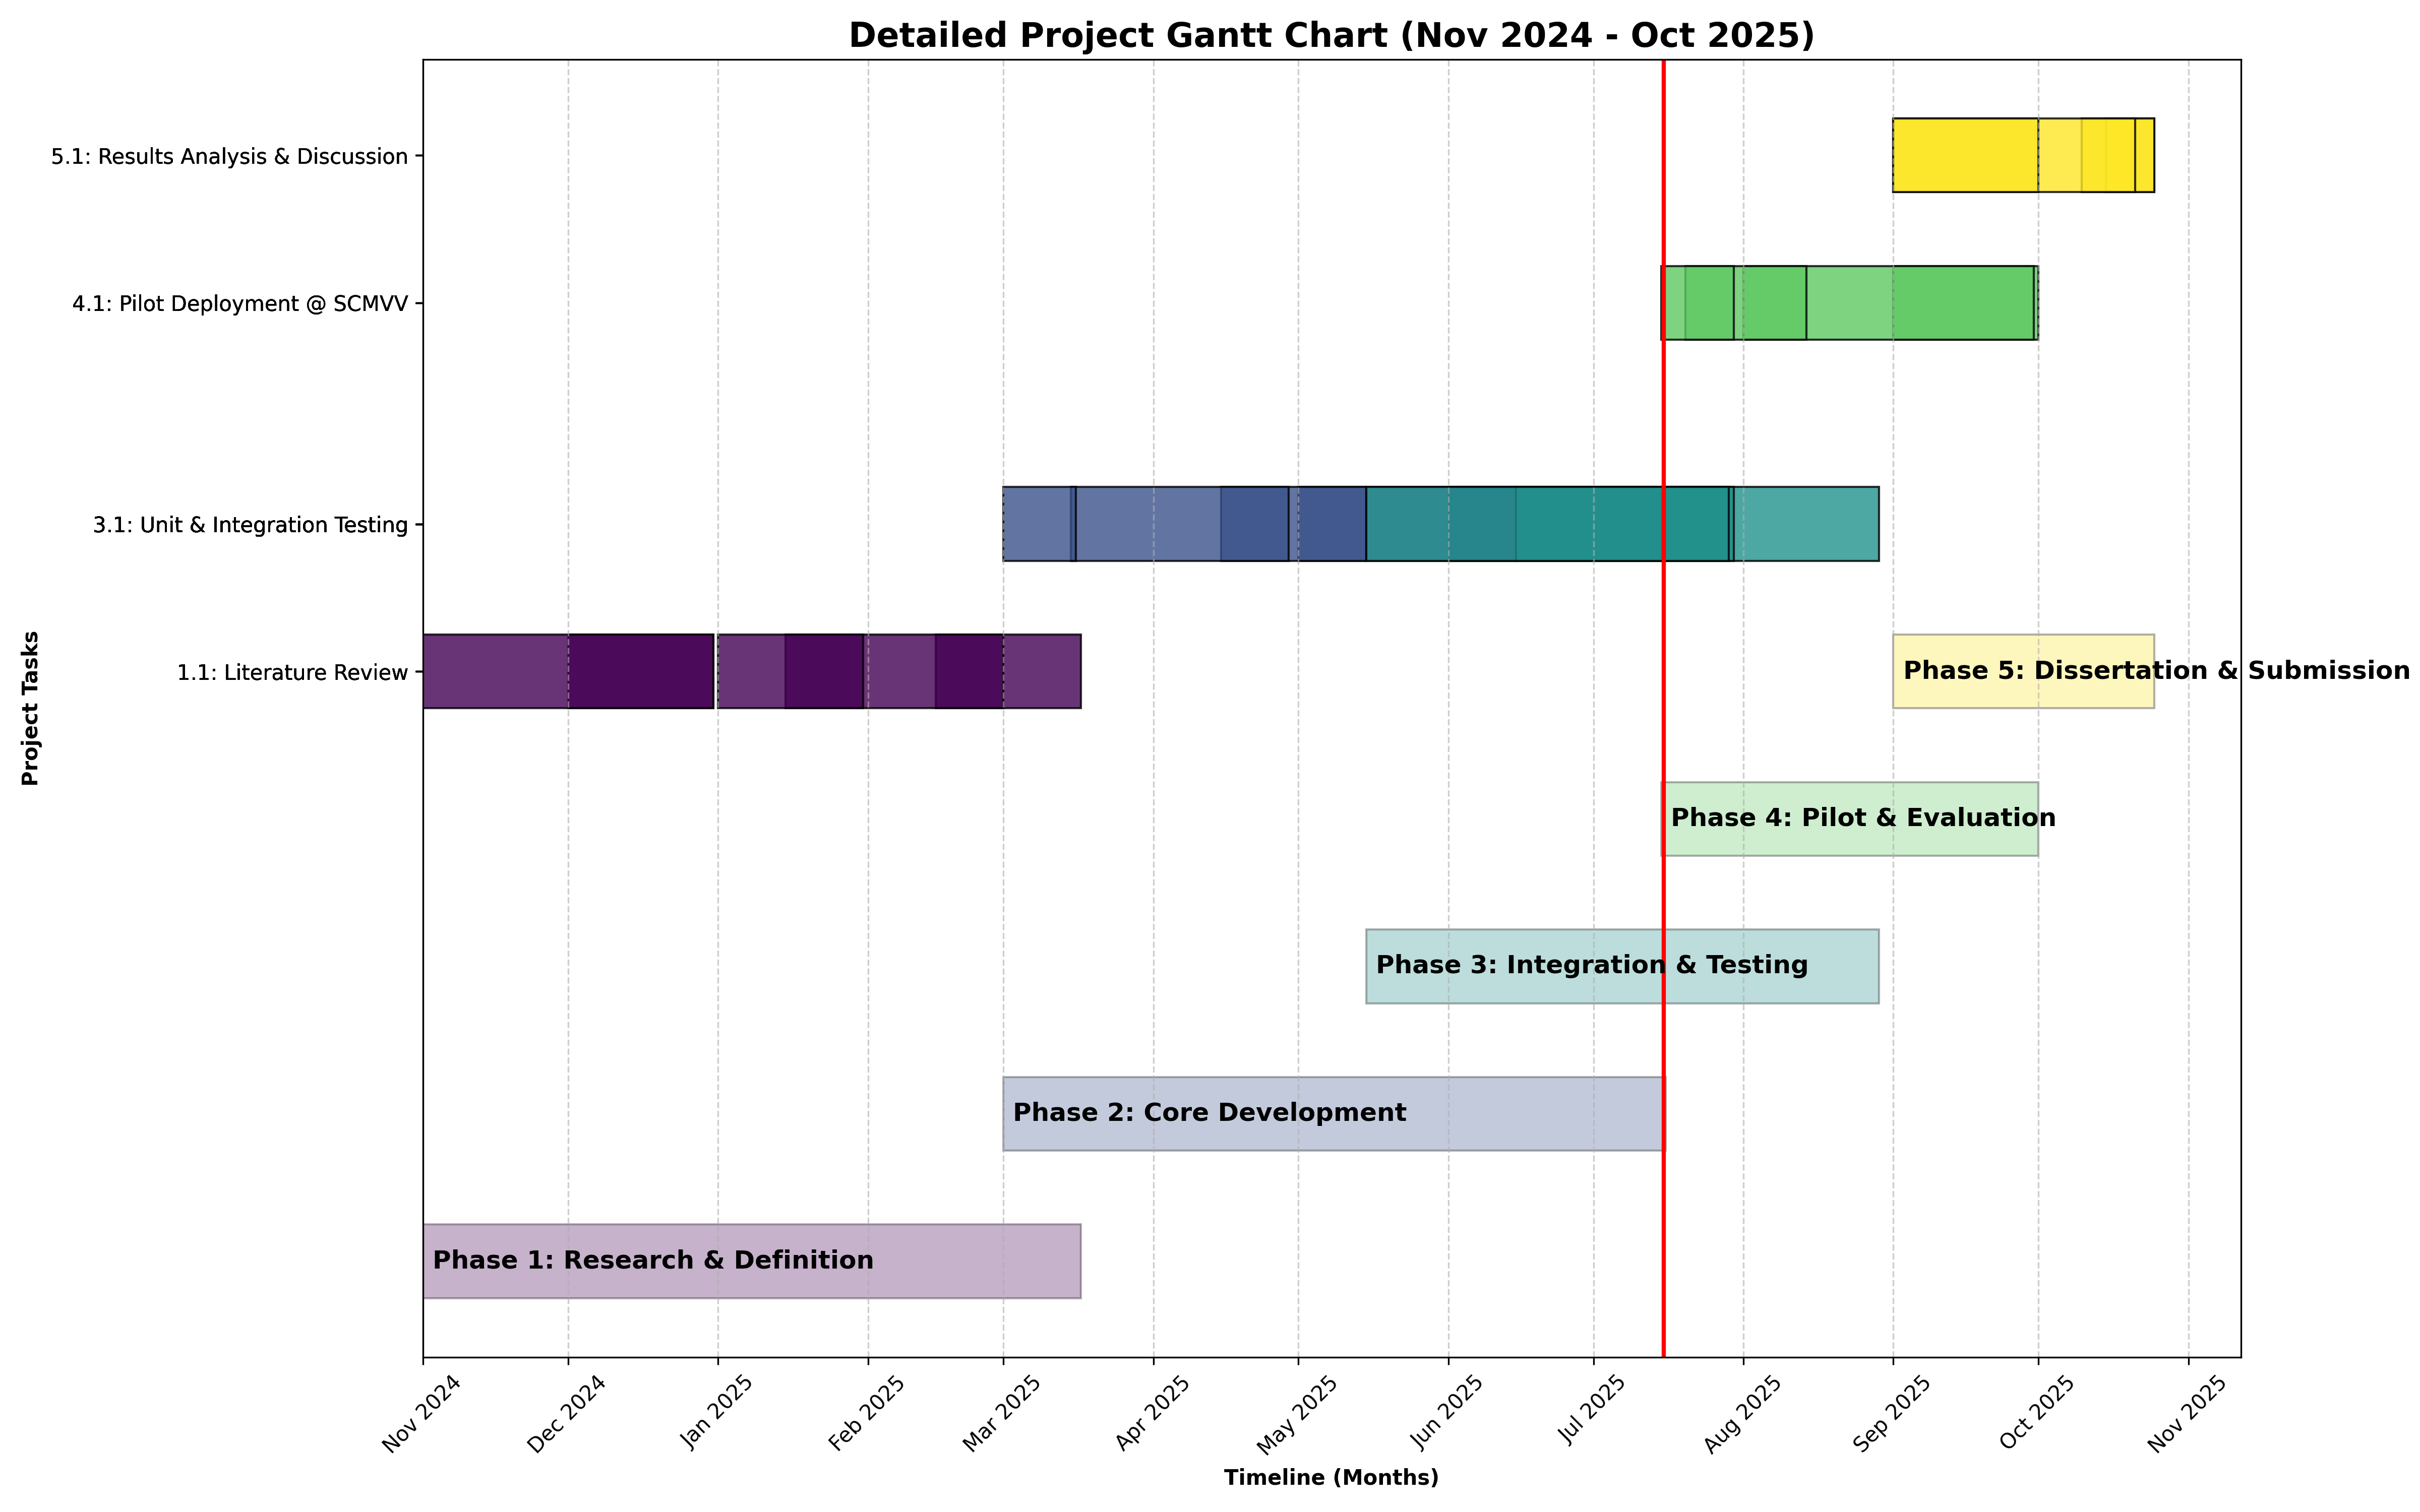
\includegraphics[width=\textwidth]{images/generated/gantt_chart_detailed.png}
    \caption{Detailed Gantt chart illustrating the 12-month project timeline, key phases, and task dependencies from November 2024 to October 2025.}
    \label{fig:gantt_chart_detailed}
\end{figure}

The initial phase, \textit{Research and Definition}, focused on establishing a solid theoretical and empirical foundation through an exhaustive literature review and an in-depth analysis of the existing clinical workflows at SCMVV. This was followed by the \textit{Core Development} phase, where the system's foundational components, including the database, security modules, and core backend logic, were implemented.

Subsequently, the \textit{Integration and Testing} phase ensured that the newly developed modules operated cohesively and could be reliably connected to existing external and legacy systems. The fourth phase, \textit{Pilot and Evaluation}, marked the transition from a development environment to a live clinical setting, where the system was deployed and rigorously evaluated based on user feedback and performance data.

The final phase, \textit{Dissertation and Submission}, was dedicated to the analysis of the collected data, the synthesis of the research findings, and the writing of this dissertation, culminating in its final submission and defense. The detailed methodological framework underpinning the execution of this plan is elaborated upon in the following chapter.

\section{Risk Analysis and Mitigation Strategies}
\label{sec:RiskAnalysis}

A proactive approach to risk management is essential for the successful execution of this project. Potential risks have been identified across four key domains: technological, project management, user adoption, and data governance. For each risk, a corresponding mitigation strategy has been developed to minimize its potential impact.

\begin{description}
    \item[Technological Risks] The primary technological risk involves integration challenges with the hospital's legacy systems, which may have outdated protocols or insufficient documentation.
    \textbf{Mitigation:} An early-stage integration analysis will be conducted, creating proxy services or "anti-corruption layers" to isolate the new system from legacy complexities. Furthermore, a phased integration rollout is planned, starting with non-critical data streams to validate the approach before full implementation.

    \item[Project Management Risks] Scope creep represents a significant risk, where the project's requirements expand beyond the initial plan, potentially delaying the timeline. Another risk is the potential for unforeseen technical challenges that consume more time than allocated.
    \textbf{Mitigation:} A stringent change control process will be implemented. All new feature requests will be formally evaluated for their impact on the project timeline and resources, requiring approval from all stakeholders. The work plan includes a 15\% buffer in each phase for unforeseen technical issues, providing a contingency to address challenges without compromising the final deadline.

    \item[User Adoption Risks] Resistance to change from healthcare professionals accustomed to existing workflows is a critical risk. If the system is perceived as difficult to use or disruptive, its adoption and, consequently, its benefits will be limited.
    \textbf{Mitigation:} A user-centered design (UCD) methodology is central to this project. Key users from different professional groups (physicians, nurses, pharmacists) will be involved throughout the design and testing phases. Comprehensive training programs and ongoing support will be provided during the pilot deployment to ensure a smooth transition.

    \item[Data Governance and Security Risks] Handling sensitive patient data introduces significant risks related to security breaches and compliance with data protection regulations such as GDPR.
    \textbf{Mitigation:} The system is being designed with a "security-by-design" approach. This includes end-to-end data encryption, robust authentication and authorization mechanisms (including SSO and role-based access control), and a complete audit trail of all data access and modifications. A formal Data Protection Impact Assessment (DPIA) will be conducted before the pilot study to ensure full compliance with all legal and ethical requirements.
\end{description} 